%%%%%%%%%%%%%%%%%%%%%%%%%%%%%%%%%%%%%%
% Multiplicative domain poster
% Created by Nathaniel Johnston
% August 2009
% http://www.nathanieljohnston.com/2009/08/latex-poster-template/
%%%%%%%%%%%%%%%%%%%%%%%%%%%%%%%%%%%%%%

\documentclass[final]{beamer}
\usepackage[scale=1.24]{beamerposter}
\usepackage{graphicx}   % allows us to import images

%-----------------------------------------------------------
% Custom commands that I use frequently
%-----------------------------------------------------------

\newcommand{\bb}[1]{\mathbb{#1}}
\newcommand{\cl}[1]{\mathcal{#1}}
\newcommand{\fA}{\mathfrak{A}}
\newcommand{\fB}{\mathfrak{B}}
\newcommand{\Tr}{{\rm Tr}}
\newtheorem{thm}{Theorem}

%-----------------------------------------------------------
% Define the column width and poster size
% To set effective sepwid, onecolwid and twocolwid values, first choose how many columns you want and how much separation you want between columns
% The separation I chose is 0.024 and I want 4 columns
% Then set onecolwid to be (1-(4+1)*0.024)/4 = 0.22
% Set twocolwid to be 2*onecolwid + sepwid = 0.464
%-----------------------------------------------------------

\newlength{\sepwid}
\newlength{\onecolwid}
\newlength{\twocolwid}
\setlength{\paperwidth}{48in}
\setlength{\paperheight}{36in}
\setlength{\sepwid}{0.024\paperwidth}
\setlength{\onecolwid}{0.22\paperwidth}
\setlength{\twocolwid}{0.464\paperwidth}
\setlength{\topmargin}{-0.5in}
\usetheme{confposter}
\usepackage{exscale}
\usepackage{listings}
\usepackage{hyperref}

%-----------------------------------------------------------
% The next part fixes a problem with figure numbering. Thanks Nishan!
% When including a figure in your poster, be sure that the commands are typed in the following order:
% \begin{figure}
% \includegraphics[...]{...}
% \caption{...}
% \end{figure}
% That is, put the \caption after the \includegraphics
%-----------------------------------------------------------

\usecaptiontemplate{
\small
\structure{\insertcaptionname~\insertcaptionnumber:}
\insertcaption}

%-----------------------------------------------------------
% Define colours (see beamerthemeconfposter.sty to change these colour definitions)
%-----------------------------------------------------------

\setbeamercolor{block title}{fg=ngreen,bg=white}
\setbeamercolor{block body}{fg=black,bg=white}
\setbeamercolor{block alerted title}{fg=white,bg=dblue!70}
\setbeamercolor{block alerted body}{fg=black,bg=dblue!10}

%-----------------------------------------------------------
% Name and authors of poster/paper/research
%-----------------------------------------------------------

\title{Can Twitter User's Moods Predict the Stock Market?}
\author{Aaron Gonzales and Adam Delora}
\institute{Department of Computer Science, University of New Mexico} 

%-----------------------------------------------------------
% Start the poster itself
%-----------------------------------------------------------
% The \rmfamily command is used frequently throughout the poster to force a serif font to be used for the body text
% Serif font is better for small text, sans-serif font is better for headers (for readability reasons)
%-----------------------------------------------------------

\begin{document}
\begin{frame}[t]
  \begin{columns}[t]            % the [t] option aligns the column's content at the top
    \begin{column}{\sepwid}\end{column}   % empty spacer column
    \begin{column}{\onecolwid}
      \begin{alertblock}{The Big Question}
        \rmfamily{If we combine semantic analysis with topic modeling, can we
        correlate our results with the market?}
      \end{alertblock}

      \vskip2ex
      \begin{block}{Background}
        \rmfamily{
          \begin{itemize}
          \item Twitter is a microblogging service with 284 million monthly
            active users who post 500 million updates (``tweets'') per day.
          \item Latent Semantic Indexing is a technique used to summarize
            words (documents) into representative ideas similar to primary
            component analysis.
          \item the AFINN semantic indexing database assigns coded valence
            values to common words to allow quantification of a set of word's
            ``mood''.
        \end{itemize}}
      \end{block}
      %\vskip2ex
      \begin{block}{Methods}
        \rmfamily{
          We collected tweets using the public Twitter Streaming RESTful API
          over 2014-10-15 \textemdash 2014-11-09 by tracking words that related
          to various tech stocks indexed by NASDAQ.           \begin{itemize}
            \item \small{Maine nurse defies Ebola quarantine order by taking bike ride.
              http://t.co/eERINkm3AQ via @indystarJ}
            \item \small{Tim Cook: Apple CEO Says 'Being Gay Is One Of God's
                Greatest Gifts' Earlier today, the chief executive of
                Apple,\ldots \url{http://t.co/zIXb2HbDmd}}
            \item \small{ Meet the Swedish twin sisters who want to be
                'identical artificial dolls' \url{http://t.co/77eA3esaQa}}
            \item \small{Last Christmas I got a black iPhone it was the
                worst Christmas present ever, I wanted a white one. I mean I'm
                not\ldots \url{http://t.co/jhP9ODs3QK}}
            \end{itemize}
            \begin{itemize}\label{keywords}
            \item \small{ 'ebola', 'aapl', 'apple', 'mac', 'tim cook', 'goog',
            'google', 'gmail', 'youtube', 'microsoft', 'msft',
            'nadella', 'twrt', 'amazon', 'amzn', 'prime', 'aws','fb',
          'facebook'}
          \end{itemize}
          NASDAQ market data was also
          collected over the same period. Tweets were preprocessed to remove
          common stopwords and latent semantic indexing was performed on
          one-hour bag-of-words bins of tweets, giving a total of xxx hours
          included in analysis. Each hour bin's LSI topics were scored using
          the AFINN database, resulting in a single number indicating semantic
          valence for each hour. This semantic data was combined with the stock
          data for visualization and analysis. A vector autoregressive (VAR)
          model was performed to assess the predictive power of the semantic
          data against the stock data.
          }
      \end{block}
    \end{column}

    \begin{column}{\sepwid}\end{column}   % empty spacer column
    \begin{column}{\twocolwid}    % create a two-column-wide column and then we will split it up later
      \begin{columns}[t,totalwidth=\twocolwid] % split up that two-column-wide column
        \begin{column}{\onecolwid}\vspace{-.69in}
          \begin{block}{Summary Statistics}
            \rmfamily{
              blah blah blah
              \vspace{0.1in}
            \begin{itemize}\justifying % the \justifying command forces the items in the list to have full justification (they don't by default)
              \item Total tweets collected: 86 million
              \item Total number of days: 25
              \item Total hour bins: 360
            \end{itemize}
            }
            Example of a LSI topic:
            \begin{lstlisting}^^J
              Put your code here.^^J
            \end{lstlisting}
            We generated 80 topics per hour using Gensim.
          \begin{figure}
          \begin{center}
            '0.748*+ 0.199*``video'' + 0.190*``my'' + -0.183*``i''
            + -0.172*``yo'' + 0.153*``me'' + 0.147*``music'' +
            -0.140*``apple'' + 0.114*``give'' + 0.113*``be''',
             '0.416*``scientists'' + 0.219*``are'' + 0.217*``about'' +
             0.216*``do'' + 0.214*``don\'t'' + 0.211*``over'' + 0.209*``say'' +
             0.209*``climate'' + 0.209*``it!'' + 0.208*``panic''',
              '0.586*``on'' + -0.315*``is'' + -0.217*``get'' + 0.165*``from''
              + -0.140*``ebola'' + -0.129*``i'' + -0.126*``google'' +
            -0.122*``it'' + -0.117*``really'' + 0.114*``liked'''
            \caption{Two exaple LSI topics}
            \label{fig:autocorrplot}
          \end{center}
        \end{figure}
          \end{block}
        \end{column}
        \begin{column}{\onecolwid}\vspace{-.69in}
          \begin{block}{Examining LSI}
            Using LSI would provide something like the following topic:
            \vspace{0.25in}
            \begin{figure}
              \begin{center}
                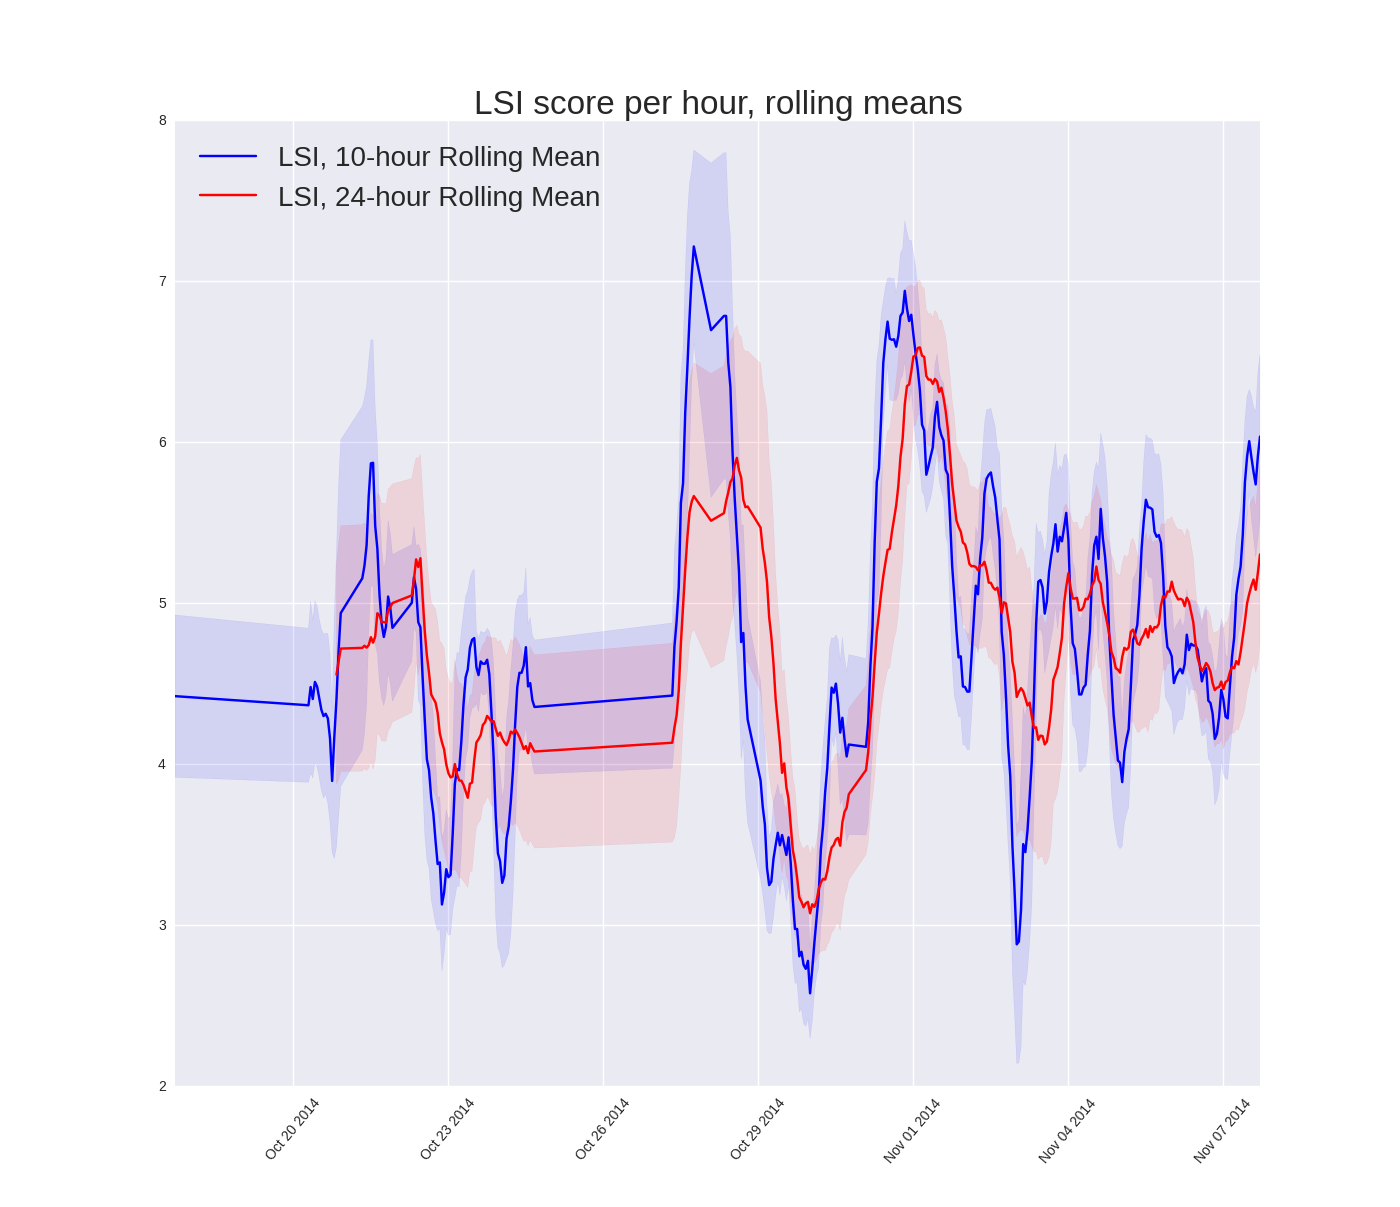
\includegraphics[width=10in]{figures/lsi_rolling_means.png}
                \caption{Rolling means of LSI score per hour over our sample.}
                \label{fig:rollingmeans}
              \end{center}
            \end{figure}
          \end{block}
        \end{column}
      \end{columns}
      \vskip2.5ex
      \begin{alertblock}{The Great Connection}  % an ACTUAL two-column-wide column
        \rmfamily{By looking at Figures 1 and 2, we expect that there might be
          some connection between correctable subsystems for a channel $\cl{E}$
          and its multiplicative domain. Indeed, one of our main results is
          that the two situations coincide when $\cl{E}$ is unital and the
        subsystem is unitarily-correctable.} \end{alertblock}
      \begin{columns}[t,totalwidth=\twocolwid]
        \begin{column}{\onecolwid}
        \begin{block}{Main Result}
          \rmfamily{\textbf{Theorem.} \emph{Let $\cl{E}$ be a unital quantum channel. Then $MD(\cl{E}) = UCC(\cl{E})$.}
          \begin{itemize}\justifying
            \item This theorem says that when we write $MD(\cl{E})$ in the form of Equation~\eqref{opalgform}, the $\cl{B}_k$'s are exactly the unitarily-correctable codes for $\cl{E}$.
            \item When $\cl{E}$ is not unital, $MD(\cl{E})$ in general only captures a subclass of the unitarily-correctable codes for $\cl{E}$.
            \item Because $MD(\cl{E})$ is easy to compute, this provides a concrete method of finding some UCCs.
          \end{itemize}}
        \end{block}
      \end{column}
      \begin{column}{\onecolwid}
        \begin{block}{Generalization}
          \rmfamily{In the same spirit as the multiplicative domain, we can define ``generalized multiplicative domains'' for channels by requiring not that the channel be multiplicative with itself, but rather that it be multiplicative with some $*$-homomorphism.
          \begin{itemize}\justifying
            \item Generalized multiplicative domains capture \emph{all} correctable codes for \emph{arbitrary} channels.
            \item Unlike the multiplicative domain, these algebras in general are very difficult to compute.
          \end{itemize}}
        \end{block}
      \end{column}
    \end{columns}
  \end{column}
  \begin{column}{\sepwid}\end{column}   % empty spacer column
  \begin{column}{\onecolwid}
    \begin{block}{Conclusions and Outlook}
      \rmfamily{This characterization provides a simple way to find all unitarily-correctable codes for unital channels and even some codes for non-unital channels. General correctable subsystems can be characterized in terms of algebras that are analogous to the multiplicative domain, though in general it is not clear how to calculate them -- further research in this area would be of great interest.}
    \end{block}
    \vskip2ex
    \begin{block}{For Further Information}
      \small{\rmfamily{For the details of our work:
      \begin{itemize}
        \item Choi, M.-D., Johnston, N., and Kribs, D. W.. Journal of Physics A: Mathematical and Theoretical \textbf{42}, 245303 (2009).
        \item Johnston, N., and Kribs, D. W., \emph{Generalized Multiplicative Domains and Quantum Error Correction} (2009, preprint).
      \end{itemize}
      \vspace{0.1in}\noindent Preprints and this poster can be downloaded from:
      \begin{itemize}
        \item www.arxiv.org
        \item www.nathanieljohnston.com
      \end{itemize}}}
    \end{block}
    \vskip2ex

    \begin{block}{References}
      \small{\rmfamily{\begin{thebibliography}{99}
      \bibitem{KLPL06} D.~W. Kribs, R. Laflamme, D. Poulin, M. Lesosky, Quantum Inf. \& Comp. \textbf{6} (2006), 383-399.
      \bibitem{zanardi97} P. Zanardi, M. Rasetti, Phys. Rev. Lett. \textbf{79},  3306 (1997).
      \bibitem{KS06} D.~W. Kribs, R.~W. Spekkens, Phys. Rev. A \textbf{74}, 042329 (2006).
      \bibitem{Cho74} M.-D. Choi, Illinois J. Math., \textbf{18} (1974), 565-574.
      \bibitem{Dav96} K.~R. Davidson, \emph{$C^*$-algebras by example}, Fields Institute Monographs, 6. American Mathematical Society, Providence, RI, 1996.
      \end{thebibliography}}}
    \end{block}
    \vskip2ex
    \begin{block}{Acknowledgements}
      \small{\rmfamily{Thank you to Dr. Abdullah Mueen for valuable
      conversations regarding our analysis and project.}} \\
      \vspace{0.5in}
      \begin{center}
        \begin{tabular}{ccc}
          
\includegraphics[width=3in]{TO.png} & \hspace{1.5in} & 
\includegraphics[width=3in]{guelph.png}
        \end{tabular}
      \end{center}
    \end{block}
  \end{column}
  \begin{column}{\sepwid}\end{column}   % empty spacer column
 \end{columns}
\end{frame}
\end{document}
